\section{Methodology}

\subsection{Datasets}
One of the major challenges in Sentiment Analysis of Twitter is to collect a labelled dataset.
Researchers have made public the following datasets for training and testing classifiers.

\subsubsection{Sanders Twitter Corpus}
This is a collection of 5,000 tweets. It was collected and annotated(!!!TODO: method of annotation) by Sanders Analytics.
It contains tweets related to four products: Apple, Microsoft, Twitter, Xyz.
The corpus has Product name, Tweet ID, and classification (positive, negative, neutral or irrelevant).
Following Twitter's privacy policy, the text, etc. can be downloaded using Twitter API.

\begin{table}[h]
\centering
	\begin{tabular}{| p{0.6\textwidth} | l | }

	\hline
		\multicolumn{1}{|c|}{Tweet} &
		\multicolumn{1}{|c|}{Classification} \\
	\hline
	\verb'S/O to @apple for replacing my phone for free...' &  \verb'positive' \\ \hline
	\verb"+1  RT @Doug_Newton: @apple PLEASE FIX \#Siri!!!!" {...}
	\verb"She can't connect to your network!!!!!!!" &  \verb'negative' \\ \hline
	\verb'Apple Users Get The official Kalifornia Cavi App' {...}
	\verb'on your Apple Device now on  - powered by @Apple' {...}
	\verb'- Download it free http://t.co/HlGnvlRw' &  \verb'neutral' \\ \hline

	\end{tabular}
\caption{Tweets}
\label{table:twt}
\end{table}

\subsubsection{Stanford Twitter}
This is a collection of 100,000 tweets. It was collected and annotated(!!!TODO: method of annotation)
by Stanford Universities' Xyz Research Group.
The corpus has Product name, Tweet ID, and classification (positive, negative, neutral or irrelevant).

\subsection{Features}
A wide variety of features can be used to build a classifier for tweets.
The baseline is feature set is bag of words / unigrams.
However, there's a lot of domain specific information present in tweets that can also be used for classifying them.
Preprocessing is needed to normalise(!!!) these features. Relevant preprocessing methods are discussed below.

\subsubsection{Pre Processing}
	\begin{description}
	\item[Emoticons]{Keyboard written pictorial representation of a facial expression,
						used to draw a receiver's attention to the temper of sender's nominal verbal communication,
						thus changing and improving its interpretation. %% REF: http://en.wikipedia.org/wiki/Emoticon
					}
	\end{description}
Emoticons are identified and replaced by a single descriptive word.
The emoticons are identified by using regular expressions.
Table \ref{table:emot} lists the emoticons currently identified.

\begin{table}[h]
\centering
	\begin{tabular}{|l|llllll|}
	
	\hline
		\multicolumn{1}{|c|}{Emoticons} &
		\multicolumn{6}{|c|}{Examples} \\
	\hline
	\verb+EMOT_SMILEY+ 	& \verb+:-)+ 	& \verb+:)+ 	& \verb+(:+ 	& \verb+(-:+ 	& \verb++ 	& \verb++ \\
	\verb+EMOT_LAUGH+ 	& \verb+:-D+ 	& \verb+:D+ 	& \verb+X-D+ 	& \verb+XD+ 	& \verb+xD+ 	& \verb++ \\
	\verb+EMOT_LOVE+ 	& \verb+<3+ 	& \verb+:*+ 	& \verb++ 	& \verb++ 	& \verb++ 	& \verb++ \\
	\verb+EMOT_WINK+ 	& \verb+;-)+ 	& \verb+;)+ 	& \verb+;-D+ 	& \verb+;D+ 	& \verb+(;+ 	& \verb+(-;+ \\
	\verb+EMOT_FROWN+ 	& \verb+:-(+ 	& \verb+:(+ 	& \verb+(:+ 	& \verb+(-:+ 	& \verb++ 	& \verb++ \\
	\verb+EMOT_CRY+ 	& \verb+:,(+ 	& \verb+:'(+ 	& \verb+:"(+ 	& \verb+:((+ 	& \verb++ 	& \verb++ \\
	\hline
	
	\end{tabular}
\caption{Emoticons}
\label{table:emot}
\end{table}

Punctuations like exclaimation can also provide important information about the sentiments of the text.
We replace every word boundary by a list of punctuations present at that pont.
Table \ref{table:punc} lists the punctuations currently identified

\begin{table}[h]
\centering
	\begin{tabular}{|l|ll|}
	
	\hline
		\multicolumn{1}{|c|}{Punctuations} &
		\multicolumn{2}{|c|}{Examples} \\
	\hline
	\verb+PUNC_DOT+ & \verb+.+ & \verb++ \\
	\verb+PUNC_EXCL+ & \verb+!+ & \verb+¡+!!! \\
	\verb+PUNC_QUES+ & \verb+?+ & \verb+¿+!!! \\
	\verb+PUNC_ELLP+ & \verb+...+ & \verb+…+!!! \\
	\hline

	\end{tabular}
\caption{Punctuations}
\label{table:punc}
\end{table}

	\begin{description}
	\item[Hashtags]{These are used to indicate trending topics. Used for both naming subjects and phrases. For example, \verb+#iPad+, \verb+#SoMuchWin+}
	\item[Handels]{Every Twitter user has a unique handle. For example, Apple Inc's handle is \verb+@Apple+}
	\end{description}
	
These features are identified using regular expressions and replaced by a single word.
This helps in decreasing the size of the feature set by (!!!) percent.
Table \ref{table:preproc} illustrates preprocessing methods.

\begin{table}[h]
\centering
		\begin{verbatim}
		S/O to @apple for replacing my phone for free...

		S/O to __HNDL_APPLE for replacing my phone for free __PUNC_ELLP
		\end{verbatim}
		\begin{verbatim}
		+1  RT @Doug_Newton: @apple PLEASE FIX #Siri!!!! 
		She can't connect to your network!!!!!!!

		+1  RT __HNDL_DOUG_NEWTON: __HNDL_APPLE PLEASE FIX __HASH_SIRI __PUNC_EXCL
		She can't connect to your network __PUNC_EXCL 
		\end{verbatim}
		\begin{verbatim}
		Apple Users Get The official Kalifornia Cavi App 
		on your Apple Device now on  - powered by @Apple
		 - Download it free http://t.co/HlGnvlRw

		Apple Users Get The official Kalifornia Cavi App 
		on your Apple Device now on  - powered by __HNDL_APPLE 
		- Download it __URL
		\end{verbatim}
\caption{Tweets: Before and After preprocessing}
\label{table:preproc}
\end{table}

\subsubsection{n-grams}
These features are identified using regular expressions and replaced by a single word.
For example the following is changed to later.

\begin{figure}[h]
\centering
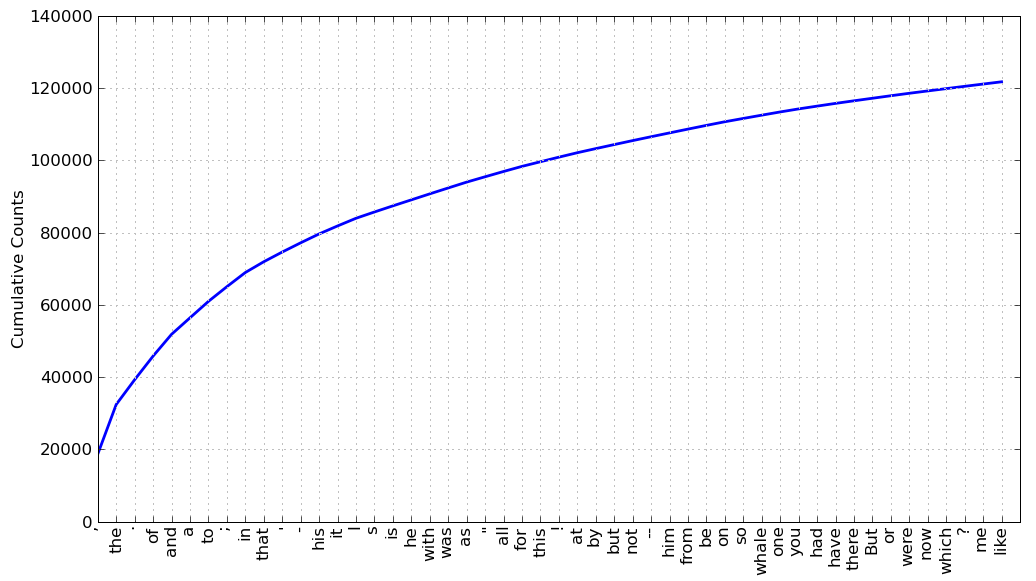
\includegraphics[width=\textwidth]{img/fdist-moby.png}
\caption{Cumulative Frequency Plot for 50 Most Frequently Words in Moby Dick: these account for nearly half of the tokens.}
\label{fig:unigram}
\end{figure}

\subsection{Experimentation}
The classifier was trained using Naive Bayes model, Maximum Entropy and Decision Tree Model.
Top classifying features are listed.

\begin{table}[h]
\centering
\begin{verbatim}
         | n   p |
         | e n o |
         | g e s |
         | a u i |
         | t t t |
         | i r i |
         | v a v |
         | e l e |
---------+-------+
negative |<.>1 . |
 neutral | .<5>. |
positive | . 3<.>|
---------+-------+

Accuracy : 0.555555555556
\end{verbatim}
\caption{Naive Bayes Statistics}
\label{naive}
\end{table}

\begin{table}[h]
\centering
Maximum Entropy Statistics here
\caption{Maximum Entropy Statistics}
\label{maxent}
\end{table}

\begin{table}[h]
\centering
Decision Tree Statistics here
\caption{Decision Tree Statistics}
\label{dtree}
\end{table}


